Herkömmliche Prozessoren verfügen über einen mehr oder weniger komplexen Befehlssatz, der es ihnen erlaubt jede beliebige Berechnung durchzuführen,
indem die Berechnung in mehrere vom Befehlssatz unterstützte Operationen aufgeteilt wird. Dadurch sind sie extrem flexibel.
Für rechenintensive Aufgaben, bei denen einige Instruktionsabfolgen sehr oft hintereinander ausgeführt werden müssen, ist dieser Ansatz jedoch nachteilig,
da der Prozessor viel Zeit benötigt, um diese komplexen Operationen zu berechnen. Um dem Abhilfe zu verschaffen, wird spezialisierte Hardware,
wie zum Beispiel Grafikkarten, Netzwerkkarten oder FPGAs eingesetzt, die besonders effizient eine bestimmte Art von Aufgabe erfüllen.
Durch die fortschreitende Digitalisierung und Vorstöße in Bereichen wie der Industrie 4.0 oder dem Internet der Dinge (IoT) wächst der Bedarf an Kleinstrechensystemen,
die für den konkreten Anwendungszweck spezielle Aufgaben übernehmen können. Diese müssen vor allem energieeffizient, klein und günstig in der Produktion sein
und müssen dabei trotzdem auch in der Lage sein, komplexere Aufgaben teilweise sogar in Echtzeit erfüllen zu können.
Ein rekonfigurierbarer Prozessor bietet hier die Vorteile der hohen Flexibilität und geringen Produktionskosten eines Off-The-Shelf Prozessors
und verbindet sie mit der hohen Spezialisierbarkeit von FPGAs, indem er mehrere kleine Blöcke an vom Entwickler konfigurierbare Logikblöcke bereitstellt,
die mit speziellen Prozessorinstruktionen gesteuert werden können. Auf diese Weise können auch sehr spezielle rechenintensive Anwendungen von kleinen Prozessorsystemen
effizient ausgeführt werden.

\subsection{FPGA}
\label{sec:fpga}
\begin{figure}
    \center
    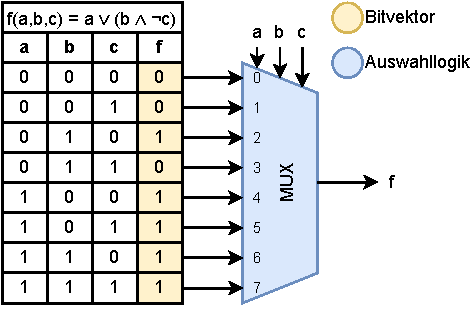
\includegraphics{images/LUT.pdf}
    \caption{Implementierung einer dreistelligen Funktion durch einen Lookup Table}
    \label{fig:fpga_lut}
\end{figure}
\textit{Field Programmable Gate Arrays} (FPGAs) sind integrierte Schaltkreise, die von sich aus keine genaue Funktion implementieren.
Stattdessen muss erst eine Schaltung "geladen" werden. Dabei macht man sich zu Nutze, dass eine n-stellige boolsche Funktion
durch einen $2^n$-Bit Vektor codiert werden kann. In Abb. \ref{fig:fpga_lut} ist zum Beispiel die Funktion
$f = A \vee (B \wedge \neg C)$ dargestellt. Der 8-Bit Ergebnisvektor wird in SRAM-Speicherzellen gehalten und durch einen 8-zu-1-Multiplexer
kann mit $A$, $B$ und $C$ das entsprechende Ergebnisbit ausgewählt werden. Diese Konstruktion wird Lookup Table (LUT) genannt.
Mehrere solcher Lookup Tables werden zusammen mit anderen Komponenten wie zum Beispiel Flip-Flops oder Recheneinheiten
wie Full-Addern zu sogenannten \textit{Configurable Logic Blocks} (CLBs) zusammengefasst. CLBs sind bereits sehr vielseitig,
aufgrund der festen Anordnung ihrer Komponenten jedoch immer noch stark eingeschränkt. Um dem entgegen zu wirken sind die CLBs
untereinander mit einem flexiblen und ebenfalls konfigurierbaren Verbindungsnetz verbunden. Auf diese Weise kann jede beliebige
Funktion realisiert werden, sofern genug CLBs zur Verfügung stehen. Neben den CLBs stellen FPGAs typischerweise auch noch andere
Komponenten bereit, die etwas speziellere oft benötigte Funktionen realisieren und die sehr viel Platz benötigen,
wenn man sie über CLBs implementiert. Dazu gehören zum Beispiel \textit{Digital Signal Processors} (DSPs).
Sie stellen Funktionen bereit, die zur Signalverarbeitung benötigt werden, können aber auch für Operationen wie Multiplikation verwendet werden.
Neben den DSPs findet man auch \textit{Block-RAM}-Einheiten (BRAM). Diese sind ähnlich wie klassischer RAM in der Lage, eine große Menge Daten zu speichern,
ohne viele LUTs zu beanspruchen. FPGAs haben gegenüber Mikroprozessoren den großen Vorteil, dass alle Funktionen, die von den Logikblöcken
realisiert werden, gleichzeitig und kontinuierlich berechnet werden. Auf diese Weise kann eine enorme Beschleunigung gegenüber einer
reinen Software-Implementierung erzielt werden, da ein Prozessor alle Berechnungen nacheinander durchführen muss.

\section{i-Core-Architektur}
\begin{figure}
    \center
    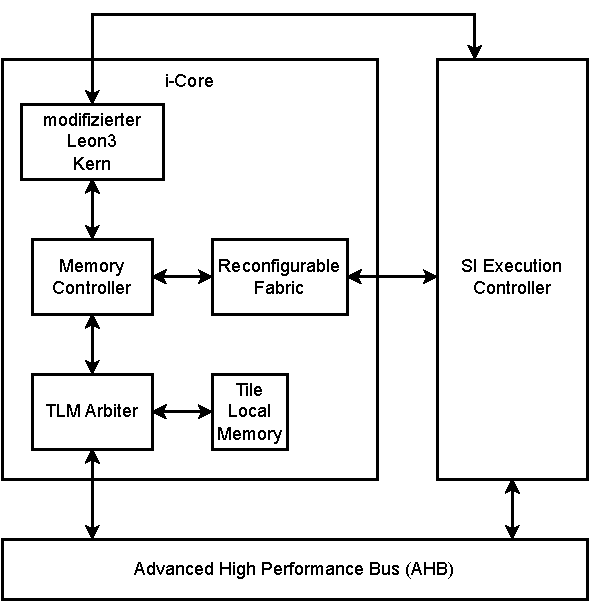
\includegraphics{images/Icore_Arch.pdf}
    \caption{Aufbau des i-Core mit Ausführungskontrolle und Reconfigurable Fabric}
	(Nachbildung aus \cite{hering2020})
    \label{fig:icore_arch}
\end{figure}
\label{sec:icore_arch}
Der i-Core ist ein von Riedlberger \cite{riedlberger2013} entwickelter rekonfigurierbarer Prozessor.
Er basiert auf der von Bauer \cite{Bauer2009} vorgestellten RISPP-Architektur, verwendet allerdings einen Leon3 als Prozessorkern.
Beim Leon3 handelt es sich um einen 32-Bit-Prozessor mit einer siebenstufigen Integer-Pipeline, der die SPARC-V8-Architektur implementiert \cite{leon3}.
Aktuell ist der i-Core vollständig auf einer Xilinx VC 707 FPGA implementiert \cite{riedlberger2015}.
Er verfügt über die \textit{Reconfigurable Fabric}, die unter anderem fünf \textit{Atom-Container} enthält.
In diese können zur Laufzeit kleine Beschleunigerblöcke (\textit{Atome}) geladen werden, mit denen ein Programm dann über
sogenannte \textit{Spezialinstruktionen} (SI) interagieren kann. Darüber hinaus besitzt der i-Core außerdem einen kleinen
Speicher mit sehr geringer Zugriffszeit, den \textit{Tile Local Memory} (TLM), der sowohl mit dem Prozessor, als auch mit der Fabric verbunden ist \cite{riedlberger2013}.

\subsection{Reconfigurable Fabric}
\begin{figure}
    \center
    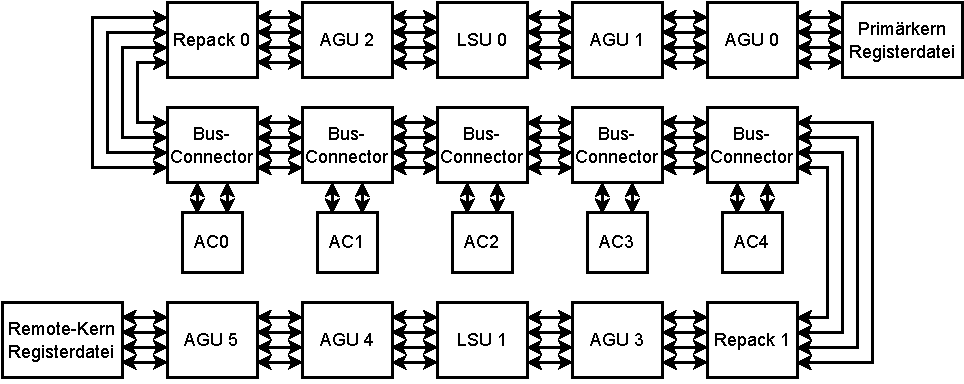
\includegraphics{images/Icore_Fabric.pdf}
    \caption{Aufbau der Reconfigurable Fabric}
	(Nachbildung aus \cite{hering2020})
    \label{fig:icore_fabric}
\end{figure}
Die \textit{Reconfigurable Fabric} enthält fünf Atom-Container (AC0 bis AC4), die zur Laufzeit rekonfiguriert werden können und in die die Beschleuniger geladen werden.
Jedes Atom hat eine Größe von 1600 LUTs, die den Beschleunigern zur Verfügung stehen. Über einen Bus-Connector sind die Atom-Container über eine Schnittstelle mit zwei Kanälen
an den Bus der Fabric angebunden, welcher insgesamt über vier Kanäle verfügt. Bei allen Kanälen handelt es sich um 32-Bit-Vollduplexkanäle.
Welche Kanäle den Atomen als Ein- und Ausgabe dienen, wird von den VLCWs der Spezialinstruktion bestimmt (siehe Abschnitt \ref{sec:special_instruction}). 
Der Bus ist außerdem segmentiert, das heißt es können auch mehrere Kommunikationen auf verschiedenen Abschnitten des gleichen Kanals stattfinden,
solange sich die Kommunikationspfade nicht physisch überlappen. Neben den Atomcontainern verfügt die Fabric
noch über weitere Komponenten wie \textit{Load-Store-Units} (LSUs), mit denen Daten aus dem TLM oder dem RAM gelesen oder geschrieben werden können.
Jede LSU besitzt eine 128 Bit Anbindung mit dem TLM, mit dem die LSU mit geringer Latenz eine große Menge Daten verarbeiten kann.
Um die gelesenen Daten zu halten, stehen den LSUs jeweils vier Puffer it jeweils 128 Bit zur Verfügung. Mit Hilfe von \textit{Address-Generation-Units} (AGUs)
können verschiedene Zugriffsmuster für die LSUs generiert werden. Zuletzt gibt es noch die \textit{Repack Units}, mit denen Daten auf dem Bus
kombiniert werden können. Wir werden sie nicht weiter benötigen, deshalb seien sie hier nur der Vollständigkeit halber kurz erwähnt.
All diese Komponenten sind ebenfalls mit dem Bus verbunden. An den Enden des Busses werden die Register des Prozessors bereitgestellt,
sodass die Fabric auf bis zu vier Argumente zugreifen kann \cite{riedlberger2013}. Die genaue Anordnung der Komponenten ist in Abbildung \ref{fig:icore_fabric} dargestellt.

\subsection{Spezialinstruktionen}
\label{sec:special_instruction}
Der i-Core stellt Spezialinstruktionen (SIs) bereit, die von Programmen benutzt werden, um die Beschleuniger zu verwenden.
Taucht eine solche Spezialinstruktion im Programmcode auf, wird die Pipeline des Prozessors angehalten und, falls notwendig,
die für den Beschleuniger benötigten Atome konfiguriert. Über den \textit{SI Execution Controller} (siehe Abschnitt \ref{sec:si_exec_ctl})
wird dann die Abarbeitung durch den Beschleuniger durchgeführt. Nachdem die Abarbeitung abgeschlossen ist, wird dann die Kontrolle wieder an den Prozessor übertragen
und die Pipeline wird fortgesetzt \cite{riedlberger2013}.

\subsection{SI Execution Controller}
\label{sec:si_exec_ctl}
Die Spezialinstruktionen sind mit VLCWs (\textit{Very Long Control Words}) mikroprogrammiert. Wird ein Beschleuniger geladen,
wird auch der Mikrocode für den Beschleuniger in den \textit{Execution Controller} geladen. Dieser hat die volle Kontrolle über die
\textit{Reconfigurable Fabric} und kontrolliert mit Hilfe der VLCWs ihre Komponenten. Jedes VLCW definiert dabei einen Kontrollschritt,
welche der Reihe nach abgearbeitet werden. Für die Atome werden von einem VLCW die Anbindung der Eingabe- und Ausgabekanäle an den Bus
bestimmt sowie ein 6-Bit Kontrollvektor. Die Funktion des Kontrollvektors kann im Atom beliebig realisiert werden. Für die LSUs wird bestimmt
welche AGU zur Adressgenerierung verwendet werden soll, welche Puffer für die Lese-/Schreiboperation verwendet werden sollen und
welche Daten aus dem Puffer an den Bus angelegt werden sollen bzw. vom Bus in den Puffer übernommen werden sollen.
Für die AGUs wird der Betriebsmodus über die VLCWs bestimmt. Es gibt sowohl Betriebsmodi für rein statische Zugriffsmuster,
die vollständig über die VLCWs bestimmt werden, als auch dynamische Modi, bei denen das Zugriffsmuster über Parameter direkt vom Datenbus bestimmt wird.
Für jede Spezialinstruktionen stehen insgesamt 256 VLCWs zur Verfügung. Um auch Programme zu realisieren,
die länger als 256 Kontrollschritte sind, sind auch rudimentäre statische Schleifen im Mikrocode möglich \cite{riedlberger2013}.

\section{Erweiterung: Dynamische Ausführung}
Um auch einen dynamischen Kontrollfluss innerhalb des VLCW-Mikrocodes zu ermöglichen, wie zum Beispiel Schleifen, die von einem Laufzeitparameter abhängen,
verwenden wir eine von Hering \cite{hering2020} entwickelte Erweiterung der VLCWs. Die Atomcontainer werden mit zwei weiteren Ausgabebits ausgestattet.
Diese können vom den Atomen des Beschleunigers beliebig implementiert werden. Um nun Sprünge realisieren zu können, werden die VLCWs um einen neuen Kontrollabschnitt erweitert.
Dieser kann benutzt werden, um Zählervariablen für Schleifen zu setzen oder Sprünge anhand von diesen Zählern durchzuführen. Es sind jedoch auch Sprünge möglich,
die nur bei bestimmten Mustern der neuen Ausgabebits der Atome genommen werden. Hierzu lässt sich im VLCW mit einer Bit-Maske codieren welche Atom-Container betrachtet werden sollen,
ob die Bedingung für alle oder nur für einen Atom-Container erfüllt sein muss, welche Vergleichsoperation auf der Ausgabe der Atom-Container durchgeführt werden soll und
zu welcher VLCW gesprungen werden soll \cite{hering2020}. Diese Erweiterung ist für die Realisierung von Hashfunktionen besonders interessant,
da die Eingabelänge für die Berechnung völlig variabel ist und so immer zur Laufzeit bestimmt werden muss, wie oft die zugrundeliegende Funktion berechnet werden muss.
Ohne diese Erweiterung wäre es nicht möglich, die vollständige Berechnung innerhalb einer einzigen Spezialinstruktion durchzuführen, sondern der dynamische Teil müsste
in Software implementiert werden und es müsste nach jeder Iteration des Beschleunigers das Zwischenergebnis gespeichert werden was, wie wir später bei der Implementierung
sehen werden, zu starken Leistungseinbußen führen würde.